%bakalarka wireframe dokumentacia

\documentclass[10pt,english,a4paper]{report}

\usepackage[english]{babel}
\usepackage[T1]{fontenc}
\usepackage[IL2]{fontenc} 
\usepackage[utf8]{inputenc}
\usepackage{graphicx}
\usepackage{url}
\usepackage{hyperref} 
\usepackage{xcolor}
\usepackage{subcaption} % For subfigures

\usepackage{booktabs}
\usepackage{longtable}
\usepackage{adjustbox}
\usepackage{float}
\usepackage[a4paper,margin=1in]{geometry}

\newtheorem{definition}{Definition}


\usepackage{cite}
\usepackage{times}
\usepackage{ragged2e}
\usepackage{amsmath}
\usepackage{amssymb} % For extra symbols, if needed
\usepackage{textcomp} % For using the backtick character

\pagestyle{headings}

\title{Who wrote that?} 

\author{Richard Čerňanský\\ Ing. Juraj Perík\\
	{\small Slovenská technická univerzita v Bratislave}\\
	{\small Fakulta informatiky a informačných technológií}\\
	{\small \texttt{xcernansky@stuba.sk}}\\
	}

\date{\small November 23, 2024} 

\begin{document}


\maketitle

\begin{abstract}
abstract abstract abstract

\end{abstract}

\chapter{Introduction}

\section{Motivation}

In this thesis, we aim to analyze the performance of our re-implemented code2vec NN model, which utilizes an attention mechanism to process concatenated inputs to classify function under a certain name. The input to this model is derived from node-to-node features of functions' Abstract Syntax Trees (ASTs). The evaluation focuses on source code snippets written in the C programming language, sourced from datasets of competitive programming events.

\section{Domain Analysis}

\section{Source code feature extraction}
Source code is essentially just a text representation of the algorithm it 
represents for the machine. In source code analysis, what we need is 
concise method on how to extract syntactic, semantic and contextual information that defines such code snippet. There are many types of representation methods like token-based, tree-based and graph based.
\cite{samoaa}. Watson in his book \cite{DanielWatson} proposes similar division, he adds character level features and provides us with exact feature definitions for each category.  What we are interested in is the tree-based representation.

This section answers the following questions:

\begin{enumerate}
    \item What techniques are utilized to process source code for extracting its unique information?
    \item What is an Abstract syntax tree?
    \item What are the possibilities for extracting features from an AST?
    \item How do we utilize the information stored in a function's AST?
    \item Why is this approach used?
\end{enumerate}

\subsection{What techniques are utilized to process source code for extracting its unique information?}


\subsection{What is an Abstract syntax tree?}
\quad Abstract syntax tree (AST) is a tree-based representation of source code, where nodes represent various elements of the source code and paths represent relationships of the structure. AST is an inseparable part of compilation process for many reasons. It is used as an intermediate representation of program utilized for optimization and generation of machine code. Nodes of the tree can be either internal (non-leaf) or leafs. Internal nodes define the program's constructs or operations for their children. Leaf nodes store the actual textual value. Let's see the following definition.
\begin{definition}
\cite{sun2023AST}
\textbf{Abstract Syntax Tree (AST).} An Abstract Syntax Tree (AST) for a method is a tuple
$\langle N, T, X, s, \delta, \phi \rangle$ where $N$ is a set of non-terminal nodes, $T$ is a set of terminal nodes, $X$ is a set of values, $s \in N$ is the root node, $\delta : N \to (N \cup T)^*$ is a function that maps a non-terminal node to a list of its children, $^*$ represents closure operation, and $\phi : T \to X$ is a function that maps a terminal node to an associated value. Every node except the root appears exactly once in all the lists of children. 
\end{definition} 

\textbf{Example of AST}

Below is an example of a simple C function and its corresponding Abstract Syntax Tree (AST):
\begin{verbatim}
int add(int a, int b) {
    return a + b;
}
\end{verbatim}

The corresponding AST is structured as follows:
\begin{verbatim}
TranslationUnit 
|--FunctionDefinition `int add(int a, int b) {`
   |--BasicTypeSpecifier `int`
   |--FunctionDeclarator `add(`
   |  |--IdentifierDeclarator `add`
   |  |--ParameterSuffix `(int a, int b)`
   |     |--ParameterDeclaration `int a`
   |     |  |--BasicTypeSpecifier `int`
   |     |  |--IdentifierDeclarator `a`
   |     |--ParameterDeclaration `int b`
   |        |--BasicTypeSpecifier `int`
   |        |--IdentifierDeclarator `b`
   |--CompoundStatement `{ return a + b; }`
      |--ReturnStatement `return a + b;`
         |--AddExpression `a + b`
            |--IdentifierName `a`
            |--IdentifierName `b`
\end{verbatim}

\subsection{What are the possibilities for extracting information from an AST?}
Features divide into 4 main kinds according to the nature of the information extracted from the Abstract Syntax Tree (AST):
\begin{itemize}
    \item \textbf{Structural} \label{item:structural} 
    Structural features capture the structural complexity of AST. These are often some numerical quantitative values like depth of the graph, number of nodes, or average branching factor of internal nodes. 
    \item \textbf{Semantic} \\
    Semantic features reflect the semantic information encoded in AST. It could be as simple as the distribution of node kinds (that are defined by the compiler that creates the AST) or the distribution of distinct root-to-leaf paths. 
    \item \textbf{Syntactic} \\
    Syntactic features describe the paradigm in which the source code is written and the logical complexity of the program. These might include the number of functions or functor structures, or the number of control flow units.
    \item \textbf{Combined} \\
    Combined features are use-case specific, and it is up to the data analyst to design the best fit solution for information extraction using the combinations and alternations of the aforementioned strategies. Combined features are also the ones that are usually used when tackling real-world problems like source code authorship attribution or function name classification.   
\end{itemize}

\subsection{How do We utilize the information stored in a function's AST?}
The problem of function name classification requires such information extraction design to capture all three of the structural, semantic and syntactic features in a number vector that could be somehow fed into a neural network classifier. Code2vec \cite{code2vec} proposes solution design that extracts so called 'path-contexts' which are encoded into vector space using the embedding values of its components. Let's see the following definitions. 

\begin{definition}
\textbf{Path context in AST}
\cite{bogomolov}
Path context is a triplet consisting of path between two leaves in a tree and the starting node's data (token value) and the ending node's data structured like this: $\langle \text{start\_node.data}, \text{path\_arr}, \text{end\_node.data} \rangle$. So essentially what path context represents is the connected leaf nodes and the path that connects them.
\end{definition}

\begin{definition}
\textbf{Path in AST}
Path is a sequence of connected nodes, specifically, what interests us is the sequence of types (kinds) of the AST internal nodes between two distinct (for our purposes leaf but can be any two nodes) nodes. 
\end{definition}

\textbf{Example of path context} \\
\label{path_context_example}
Below is an example of a path context between a node with data `a` and `BasicTypeSpecifier` node `int` 
(of the branch with data `int b`) derived from the Abstract Syntax Tree (AST) that we constructed earlier in the example:

\begin{verbatim}
⟨ 'a', (IdentifierName (up), AddExpression (up), ReturnStatement (up), 
       CompoundStatement (up),
       FunctionDefinition (down), FunctionDeclarator (down), 
       ParameterSuffix (down), ParameterDeclaration (down), 
       BasicTypeSpecifier (down), 'int' ⟩
\end{verbatim}

\subsubsection{Source code represented as a bag of path contexts}
\quad Finally, after extracting the path contexts between all the distinct nodes, we have a representation almost suitable as input for the neural network classifier. The only step that is left is to encode (convert) the context into numerical vectors. For this, we will use mapping function i.e. vocabularies for each of unique leaf\_node.data,
tuple(path\_from\_node\_to\_node),
and also for the output - all the names of our training dataset functions to their unique indices (if the name of function in test dataset was not seen in training dataset we ignore such prediction of classifier).    
This encoding allows us to map the indices to the embedding space. The embeddings of the components of the path context are then concatenated and used as raw numerical value input for the neural network. 

\subsection{Why is this approach used?}
It has shown that the tree traversal that is incorporated in the path-context successfully captures the structural, syntactic and semantic value of the source code\cite{alon}. The problem of assigning function names using code2vec model
can be stated as learning the information connection between the path contexts and the function names. It is important to note that \textbf{not all path context contribute with the same informative value} to the resulting prediction of the classifier. That is why \textbf{Attention mechanism} \cite{attention} is added to the network to give the path contexts in the function's bag their corresponding weight when predicting the name. This way we can focus on the important path contexts that differentiate syntactically closely related functions from one another.


\chapter{Re-implementation of code2vec NN classifier}

\section{Exploratory data analysis}
\label{item:EDA}
The dataset of functions used to train the model consists of extracted C language solutions of the Google Code Jam and Codeforces programming contests. The datasets of Google Code Jam is available on this link and Codeforces on this link.

\subsection{The Nature of the Data}
As the dataset originates from competitive programming contests, its characteristics align with the expected patterns of this domain. However, there are certain limitations and challenges that must be considered when working with such data. Based on our observations, the following points should be carefully evaluated:

\begin{enumerate}
    \item \textbf{Duplicate Entries:} 
    \label{item:duplicate_entries} 
    In programming competitions, where competitors often use template 
    helper functions, it is important to check function code strings 
    for duplicates to ensure that identical functions are not included 
    multiple times in the dataset.

    \item \textbf{Outliers:} 
    \label{item:outliers}
    The presence of abnormal functions from source code submissions may impact the analysis and model performance. These include:
    \begin{enumerate}
        \item \textbf{Extremely Short or Long Functions:} 
        \label{item:short_long_functions}
        Functions that are either unusually short or excessively long may introduce noise into the dataset and require special handling. For model predicting function names, it would be the best if function follows single-responsibility principle. (some ref would be appropriate i guess)
        
        \item \textbf{Poorly Named Functions:} 
        \label{item:poorly_named_functions}
        Inconsistent or non-descriptive function names can reduce the information gain for the model and negatively affect results. This task is, however, very difficult to address, as it is challenging for a machine to evaluate the descriptive meaning of a function name. When fetching the code snippets from the datasets, we applied a filter to filter out functions with names like 'main' and 'solve', because these names unquestionably do not provide any insight into the functionality.

        \item \textbf{Highly Complex Functions:} 
        \label{item:complex_functions}
        Functions with excessive complexity can be challenging to analyze and may contain logical circles or recursive patterns in extended representations like call graphs or control flow graphs. While an AST is acyclic by definition, complex functions with recursion, indirect function calls, or unconventional control flows may create logical loops that complicate the analysis and interpretation.

        \item \textbf{Functions Violating the Single Responsibility Principle:} 
        \label{item:single_responsibility}
        Functions that perform multiple unrelated tasks with names that do not capture all of them can be problematic for the model to evaluate the function correctly, which may lead to decreased accuracy.

        \item \textbf{Functions with Rarely Occurring Names:} 
        \label{item:rare_names}
        Rare function names present a challenge for the model, as the limited number of occurrences provides insufficient examples for the model to effectively distinguish them from similar functions with different names.
    \end{enumerate}
\end{enumerate}

An initial analysis of the function data can involve visualizing distributions of quantitative features (f.e. function names).

\subsubsection{Function name frequency}
\begin{figure}[H]
    \centering
    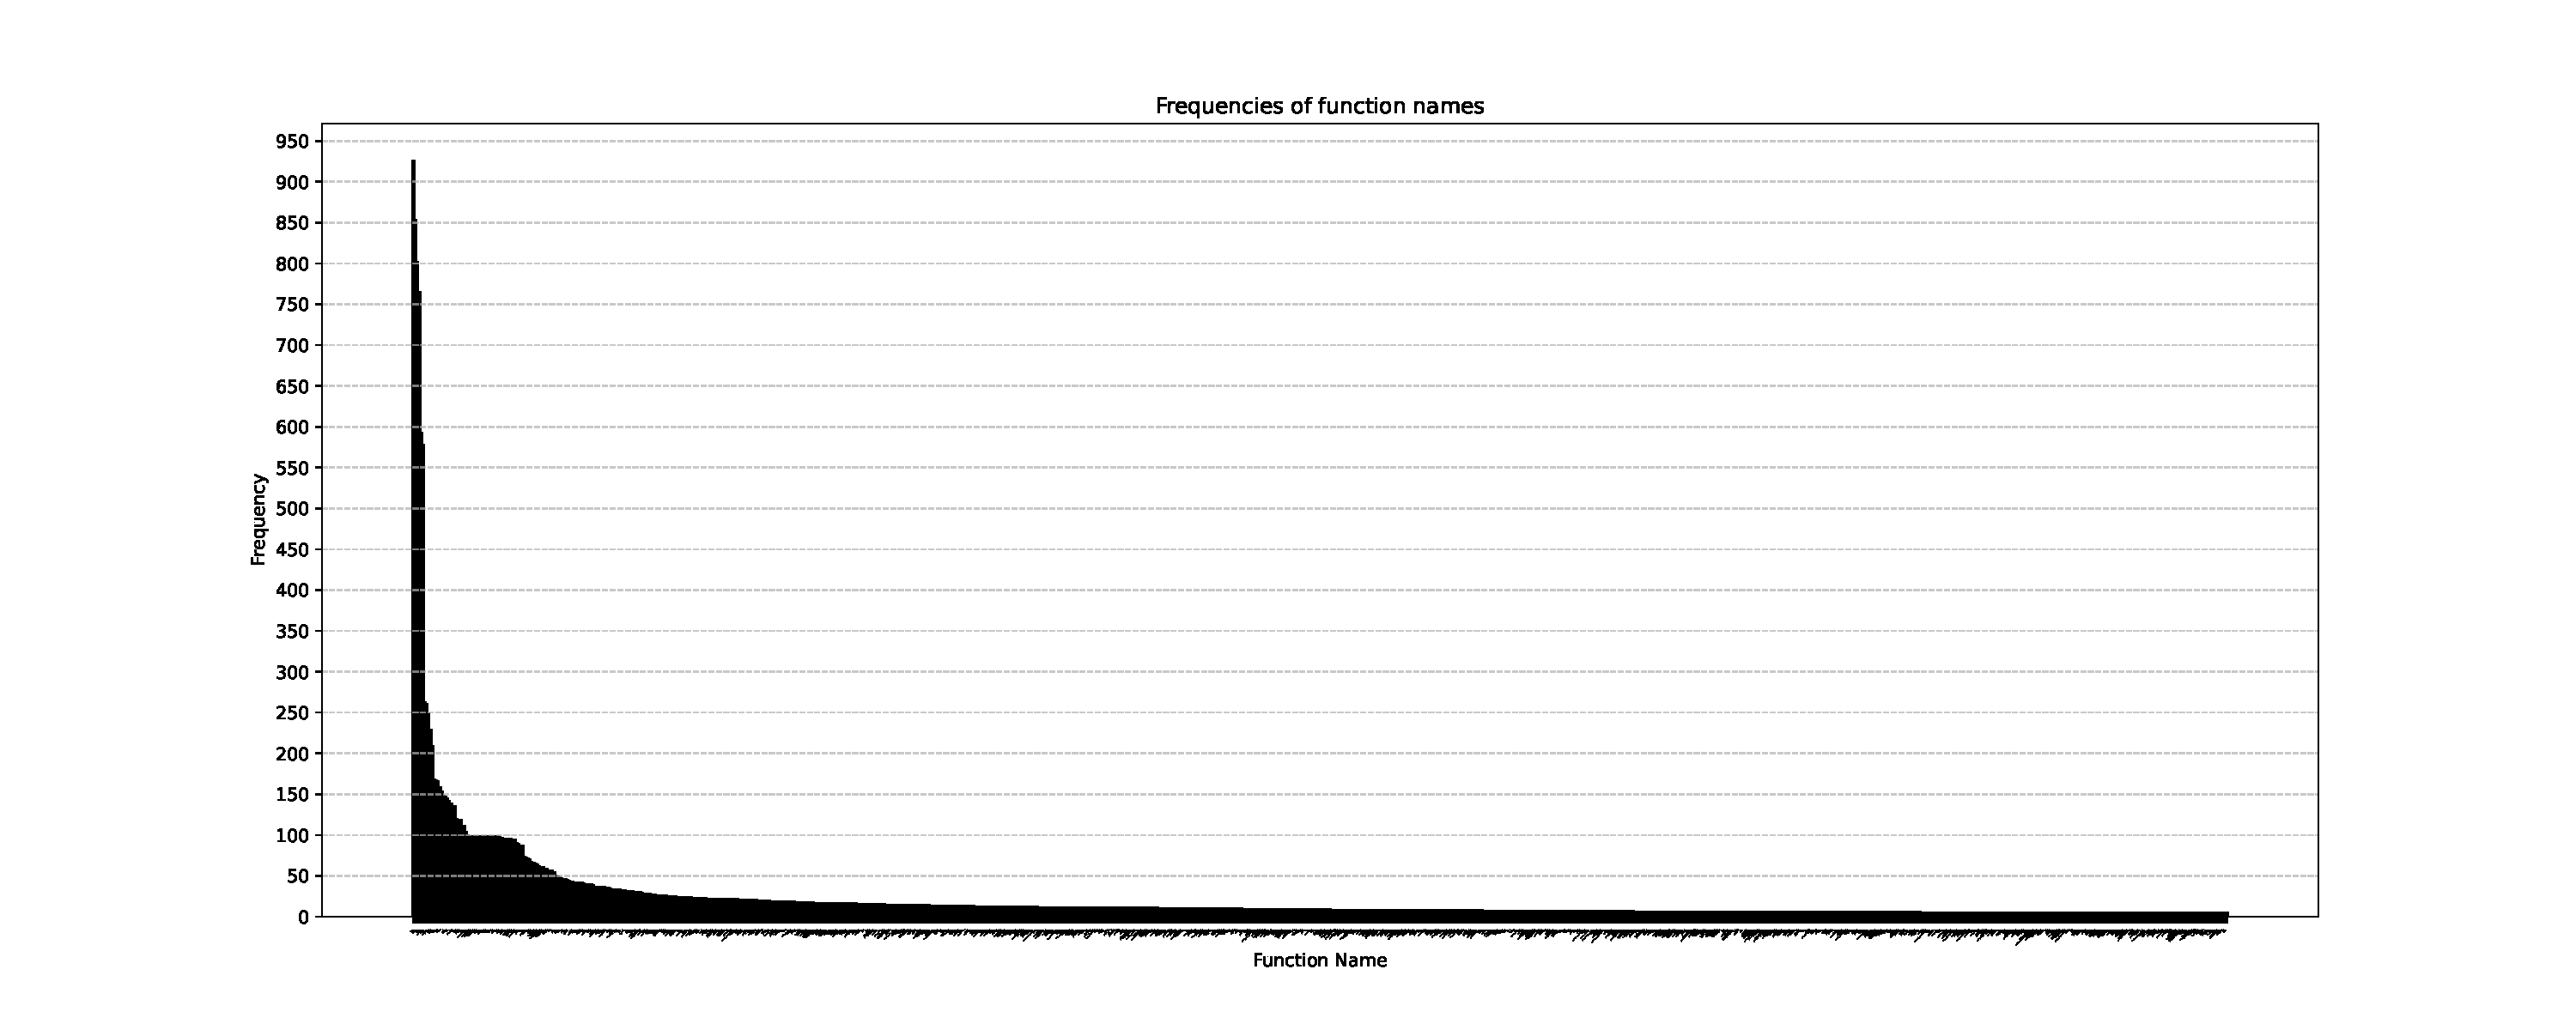
\includegraphics[width=16cm, height=9cm]{figures/functionsASTs_merged_freq_histogram.pdf} 
    \caption{Distribution of function name frequencies.}
    \label{fig:func_freq_merged}
\end{figure}

The plot reveals a long-tailed distribution of function name frequencies, with a few names occurring very frequently and many appearing rarely, but this view is inherently influenced by sorting the data by frequency. This skewed distribution highlights the dominance of common names and the sparsity of unique ones, which could introduce bias and pose challenges for machine learning models. Consequently, it is not possible to see the true underlying distribution of the data. To evaluate whether the distribution is normal (or follows another pattern), we would need to analyze the raw, unsorted frequency data through statistical normality tests.

\paragraph{Shapiro-Wilk Normality Test Results}
The Shapiro-Wilk test was applied to detect whether the data follows a normal distribution. The results are summarized below:

\begin{table}[h!]
    \centering
    \caption{Shapiro-Wilk Test Results for Function Name Frequencies}
    \label{tab:shapiro_wilk_names}
    \begin{tabular}{|c|c|c|}
        \hline
        \textbf{Statistic} & \textbf{P-value} & \textbf{Conclusion} \\
        \hline
        W = 0.2354 & $1.5252 \times 10^{-52}$ & Data is not normally distributed ($p < 0.05$) \\
        \hline
        \textbf{Mean} & \textbf{Standard Deviation} & \textbf{---} \\
        \hline
        22.7430 & 65.4305 & --- \\
        \hline
    \end{tabular}
\end{table}


\subsubsection{Function length measured in tokens}

Another basic feature that describes characteristic of data is the length of a function. There are multiple ways to represent such length when observing source code features, for now, we chose 
to just split by the whitespace characters and count the number of words.

\begin{figure}[H]
    \centering
    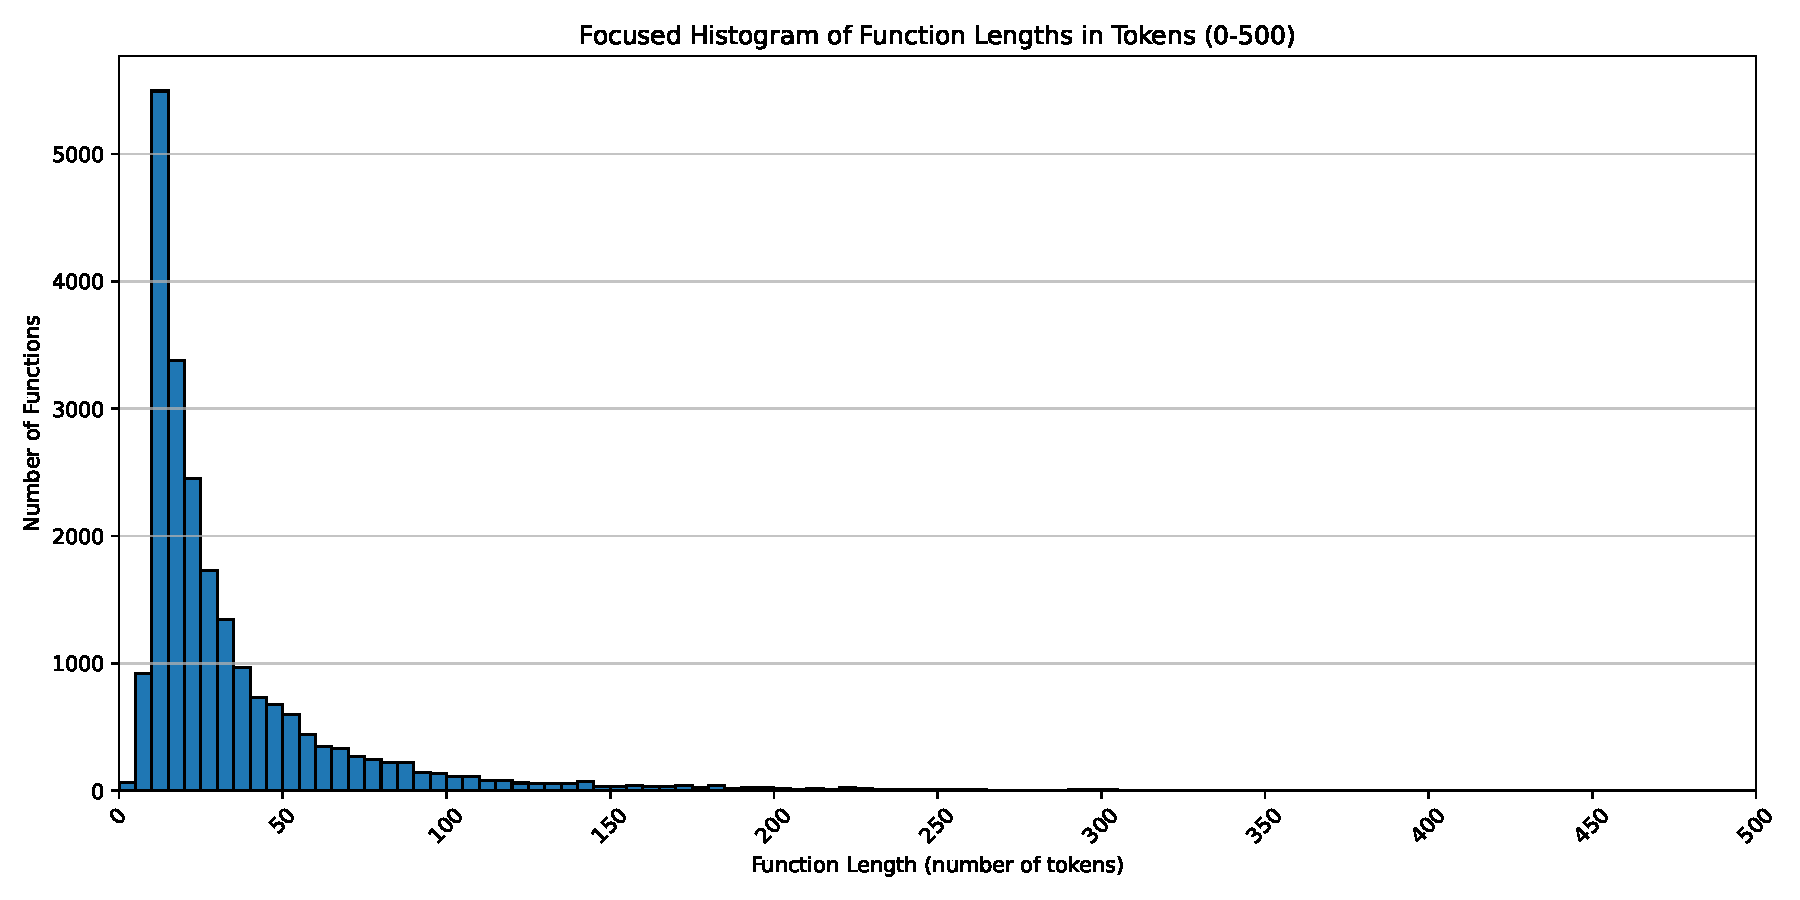
\includegraphics[width=16cm, height=9cm]{figures/FOCUSED_functionsASTs_merged_length_histogram.pdf} 
    \caption{Distribution of function lengths measured in tokens.}
    \label{fig:func_lengths_distr_merged}
\end{figure}


\begin{table}[h!]
    \centering
    \caption{Kolmogorov-Smirnov Test Results for Number of Tokens}
    \label{tab:kolmogorov_smirnov_tokens}
    \begin{tabular}{|c|c|c|}
        \hline
        \textbf{Statistic} & \textbf{P-value} & \textbf{Conclusion} \\
        \hline
        KS = 0.2482 & $0.0000 \times 10^{0}$ & Data is not normally distributed ($p < 0.05$) \\
        \hline
        \textbf{Mean} & \textbf{Standard Deviation} & \textbf{---} \\
        \hline
        36.6910 & 45.8380 & --- \\
        \hline
    \end{tabular}
\end{table}

\subsubsection{Function's AST Depth}

The distribution of AST depth is a useful metric for describing the data
to understand the structural complexity of the dataset \ref{item:structural}.

\begin{figure}[H]
    \centering
    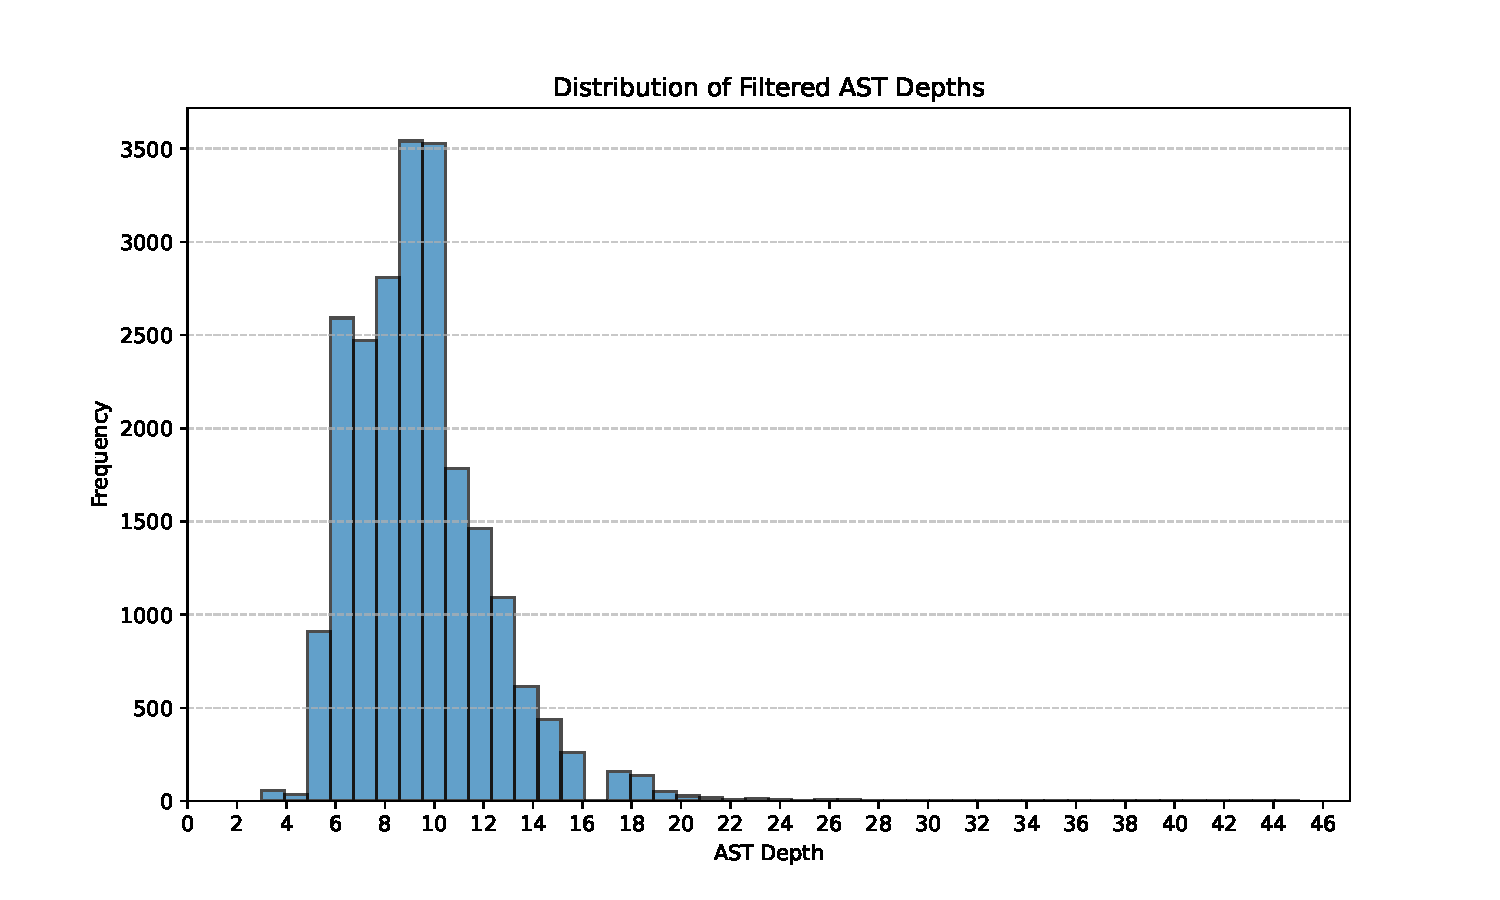
\includegraphics[width=16cm, height=9cm]{figures/ast_depths_merged.pdf} 
    \caption{Distribution of function's AST depths.}
    \label{fig:func_lengths_distr_merged}
\end{figure}

\begin{table}[h!]
    \centering
    \caption{Kolmogorov-Smirnov Test Results for AST Depths}
    \label{tab:kolmogorov_smirnov_depths}
    \begin{tabular}{|c|c|c|}
        \hline
        \textbf{Statistic} & \textbf{P-value} & \textbf{Conclusion} \\
        \hline
        KS = 0.1371 & $0.0000 \times 10^{0}$ & Data is not normally distributed ($p < 0.05$) \\
        \hline
        \textbf{Mean} & \textbf{Standard Deviation} & \textbf{---} \\
        \hline
        9.3679 & 2.8933 & --- \\
        \hline
    \end{tabular}
\end{table}

\subsubsection{Function's AST Number of nodes}

Similar to the AST Depth, AST's Number of nodes also retains information
about structural complexity.

\begin{figure}[H]
    \centering
    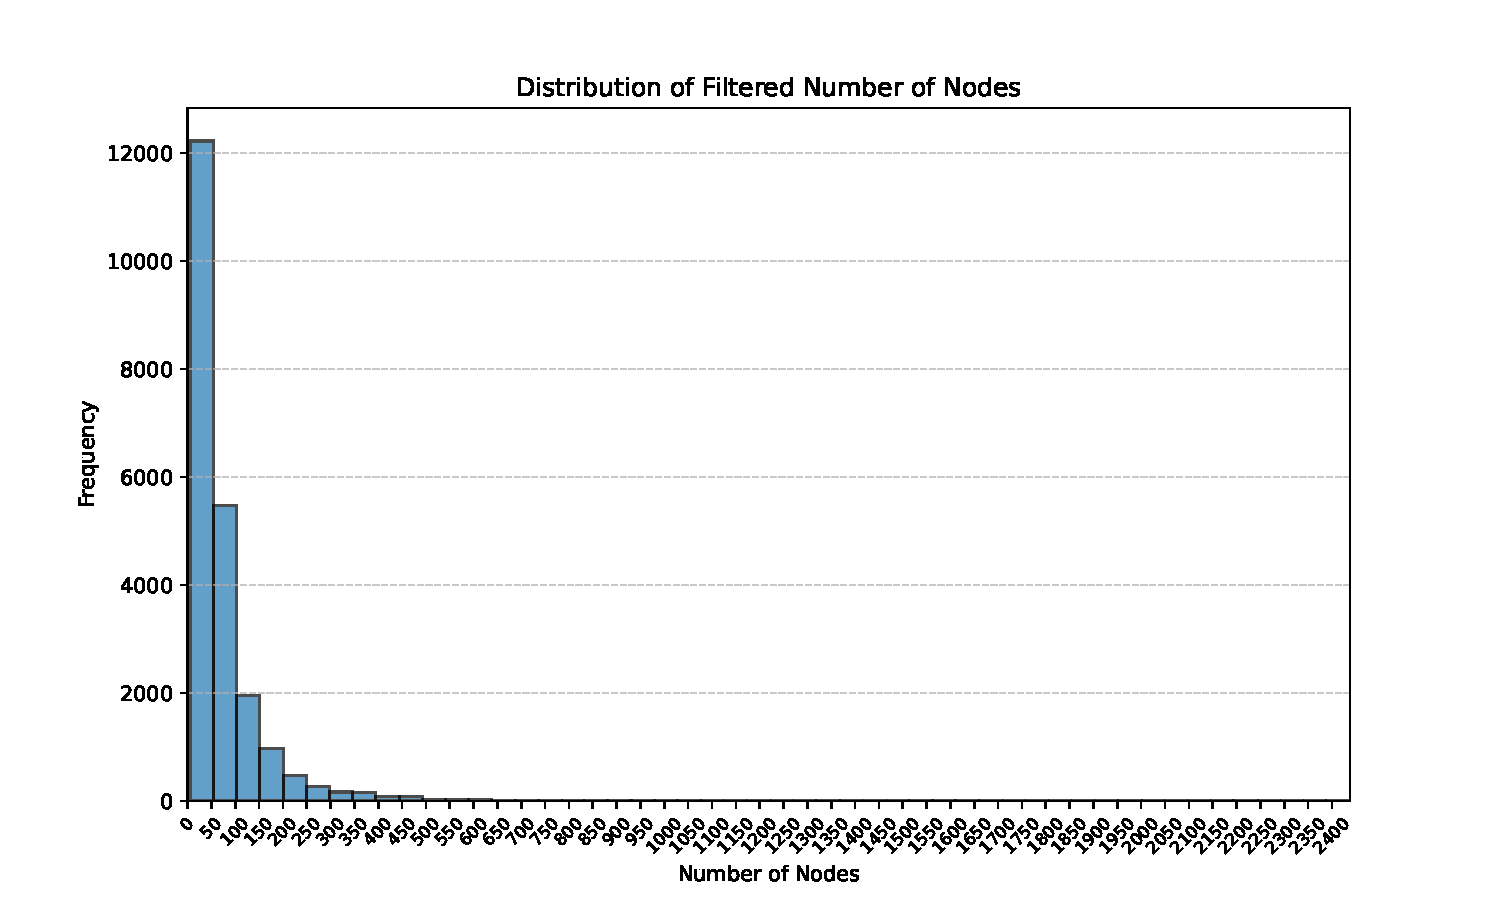
\includegraphics[width=16cm, height=9cm]{figures/num_nodes_merged.pdf} 
    \caption{Distribution of function's AST Number of nodes.}
    \label{fig:func_lengths_distr_merged}
\end{figure}

\begin{table}[h!]
    \centering
    \caption{Kolmogorov-Smirnov Test Results for Number of Nodes}
    \label{tab:kolmogorov_smirnov_nodes}
    \begin{tabular}{|c|c|c|}
        \hline
        \textbf{Statistic} & \textbf{P-value} & \textbf{Conclusion} \\
        \hline
        KS = 0.2484 & $0.0000 \times 10^{0}$ & Data is not normally distributed ($p < 0.05$) \\
        \hline
        \textbf{Mean} & \textbf{Standard Deviation} & \textbf{---} \\
        \hline
        76.7331 & 96.9949 & --- \\
        \hline
    \end{tabular}
\end{table}

\subsubsection{Key statistics for path-context based approach}
When working with NN classifier, we need to know the exact dimensions for our 
inputs' embedding matrices. Following metrics describe the sizes of vocabularies
that encode the natural-language based features to the numerical ones.


\begin{table}[h!]
    \centering
    \caption{Key statistics for path-context based approach}
    \label{tab:function_ast_summary}
    \begin{tabular}{|l|c|}
        \hline
        \textbf{Metric} & \textbf{Count} \\
        \hline
        Number of tags (function names) in total & 970 \\
        \hline
        Number of unique terminal node Data & 10055 \\
        \hline
        Number of unique node-to-node paths & 40520 \\
        \hline
        Number of unique path-contexts & 723003 \\
        \hline
    \end{tabular}
\end{table}

\subsubsection{EDA conclusion}

\subsection{Data preprocessing}
Having the data available in .csv tables format, we must have first deal with the filtering the necessary rows (solutions written in C language), transforming this code to ASCII AST using psycheC compiler. From the ASCII output of the command \textit{cnip -l -C -d file\_path} is actual
AST constructed and each function retrieved one at a time and saved (with corresponding metadata) in .ndjson as a single json line.

In the entire training pipeline, there are multiple stages where some of the above-mentioned challenges are resolved.

\begin{enumerate}
    \item \textbf{Duplicate Entries:} These are checked in the initial  stage of loading the data from task submissions in .csv into .ndjson files of function ASTs (one per line)
    \item \textbf{Poorly Named Functions:} In the script \textit{home/training\_pipeline/analysis/data\_drops\_and\_analysis.py} we perform dropping of functions that we considered poorly named after seeing the frequency distribution of the names.
    \item \textbf{Functions with Rarely Occurring Names:}  In the script \textit{home/training pipeline/analysis/data drops and analysis.py} we also perform dropping of functions whose names have lower frequency than 5 for stratification purposes (and also model performance).
    \item \textbf{Extremely long or short functions:} We are interested on how the model will
    perform when the data is cleaned from outliers in the context of function length in tokens.
\end{enumerate}


\section{Model Architecture}
In this section, we would like to provide an explanation of the model that was used to process the data and perform the predictions that are observed. This includes a detailed description of the architecture, the reasoning behind the choice of components, and the methodology employed for training and evaluation.

\section*{Model: "functional"}
As stated before, we decided to use the Attention based neural network classifier to predict C function name from 
its source code. The model is constructed using tensorflow.keras framework.

\subsection{Inputs}
The model has 3 input layers. One for each part of the path context \ref{path_context_example} and they are represented as 
vectors of indices to their respective vocabularies. The shape is decided by the maximum
number of distinct path contexts from the set of all functions in our dataset (the missing values are 
padded with zeros).

\subsection{Input embeddings}
For each input layer there is also corresponding embedding layer and the embeddings are obtained 
using the numerical index representations. Then they are concatenated into one single vector
of dimensions (1, 3d) where d is the dimension of single embedding row. 

\subsection{Dense layer}
The concatenated vector is then multiplied with weight matrix of dimensions $(y, 3d)$ to obtain
vector of dimension $y$, where $y$ is the size of tags set. Tanh function is applied to this 
transformed vector to introduce non-linearity.

\subsection{Attention-weight mechanism}
Attention weight vector is then applied to get the portion (importance) of each path context
by multiplying the attention weight $a_i$ with path context $c_i$ to get the vector $v_a$.  

\subsection{Softmax}
The final vector of probabilities is then obtained by multiplying each tag's entry in 
embedding layer of tags $(y, 1)$ with the vector $v^T$ $(1,y)$ and applying the softmax 
over all the tags in tag set. \\ \\
This foward process is depicted in the following flowchart:

\begin{figure}[H]
    \centering
    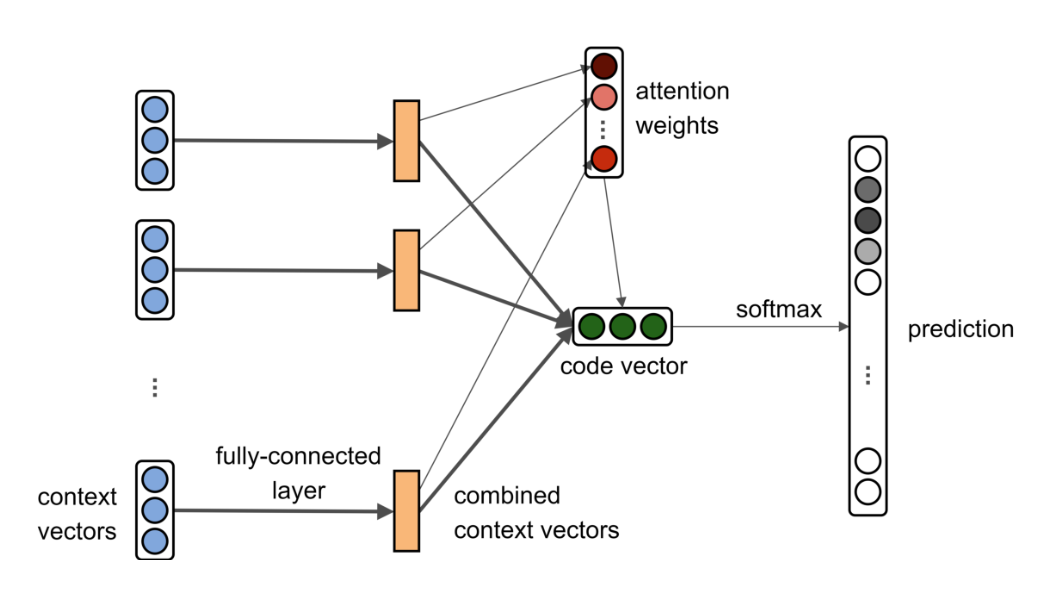
\includegraphics[width=12cm, height=7cm]{figures/code2vec_model_visual.png} 
    \caption{Code2vec \cite{code2vec} neural network model flowchart.}
    \label{fig:func_lengths_distr_merged}
\end{figure}


The model architecture is displayed in detail below in the table.
\begin{longtable}{|p{4cm}|p{5cm}|r|p{4cm}|}
\hline
\textbf{Layer (type)} & \textbf{Output Shape} & \textbf{Param \#} & \textbf{Connected to} \\
\hline
\endfirsthead
\hline
\textbf{Layer (type)} & \textbf{Output Shape} & \textbf{Param \#} & \textbf{Connected to} \\
\hline
\endhead
value1\_input (InputLayer) & (None, 723003) & 0 & - \\
\hline
path\_input (InputLayer) & (None, 723003) & 0 & - \\
\hline
value2\_input (InputLayer) & (None, 723003) & 0 & - \\
\hline
value\_embedding (Embedding) & (None, 723003, 128) & 1,081,216 & value1\_input[0][0], value2\_input[0][0] \\
\hline
path\_embedding (Embedding) & (None, 723003, 128) & 3,828,992 & path\_input[0][0] \\
\hline
concatenate (Concatenate) & (None, 723003, 384) & 0 & value\_embedding[0][0], path\_embedding[0][0], value\_embedding[1][0] \\
\hline
dense (Dense) & (None, 723003, 128) & 49,280 & concatenate[0][0] \\
\hline
dense\_1 (Dense) & (None, 723003, 1) & 129 & dense[0][0] \\
\hline
weighted\_context\_layer (WeightedContextLayer) & (None, 128) & 0 & dense\_1[0][0], dense[0][0] \\
\hline
tag\_embedding\_matrix\_layer (TagEmbeddingMatrixLayer) & (None, 740) & 94,720 & weighted\_context\_layer[0] \\
\hline
softmax (Softmax) & (None, 740) & 0 & tag\_embedding\_matrix\_layer \\
\hline
\end{longtable}

\noindent \textbf{Total params:} 5,054,337 (19.28 MB) \\
\textbf{Trainable params:} 5,054,337 (19.28 MB) \\
\textbf{Non-trainable params:} 0 (0.00 B)


\section{Training pipeline}

\subsection{Directory structure}
The training pipeline of this project is defined in the directory \texttt{./training\_pipeline:}

\begin{figure}[H]
    \centering
    \begin{minipage}{\textwidth}
    \ttfamily % Use monospaced font
    \textbf{training\_pipeline} \\
    |-- \textbf{analysis} \\
    |-- \textbf{data\_ndjson} \\
    |-- \textbf{extract\_functions} \\
    |   |-- \textbf{psychec} \\
    |   |-- \textbf{tmp} \\
    |   |-- AsciiTreeProcessor.py \\
    |   |-- main.py \\
    |   |-- Node.py \\
    |   |-- NodeTree.py \\
    |-- \textbf{trained\_models} \\
    |   |-- vocabs\_*.pkl \\
    |   |-- trained\_model\_*.h5 \\
    |-- aggregated\_avg.py \\
    |-- AttentionNNClassifier.py \\
    |-- consts.py \\
    |-- generate\_vocabs.py \\
    |-- NodeToNodePaths.py \\
    |-- stratifiedKFold.py \\
    |-- test\_one.py \\
    |-- testing\_model.py \\
    |-- train\_valid\_strat.py \\
    \end{minipage}
    \caption{Directory structure of the training pipeline (folders in bold).}
    \label{fig:training_pipeline_structure}
\end{figure}


\begin{itemize}
    \item \textbf{analysis :} This folder contains folders for EDA, training, validation
    and testing metrics plots. There is also a script for data preprocessing.

    \item \textbf{data\_ndjson :} This folder serves as the storage for all the .ndjson files
    containing AST data, whether it is the initial datase, preprocessed dataset or temporary stratificated datasets
    that are created during the pipeline.

    \item \textbf{extract\_functions :} Here the initial datasets of ASTs (and their metadata) constructed from C source code snippets from GCJ and Codeforces
    are extracted using the script \textit{main.py}. The other files are definitions of classes and helper functions 
    for this extraction 
    \item \textbf{extract\_functions/psychec :} This folder is cloned Psyche-C project \cite{psychec}. Psyche-C is a compiler frontend for the C language that provided us with AST construction.

    \item \textbf{trained\_models :} As you can see in the figure \ref{fig:training_pipeline_structure} the files in this folder with asterisk in their name a represent all the vocabs and trained models.


\end{itemize}

\subsection{Pipeline Execution: Workflow and Training Process}

This subsection explains the data pipeline through numbered steps to 
illustrate the complete function name classification process, from data
 extraction to model evaluation. These are the steps in the workflow:

 \begin{enumerate}
    \item Build and compile \texttt{psychec} for C code snippet AST generation. It is able to provide structural inference for incomplete code.

    \item Run \texttt{extract\_functions/main.py} to generate \texttt{.c} functions ASTs in \texttt{.ndjson} format (AST features as metadata included).

    \item Execute \texttt{data\_drops\_analysis.py} to drop functions with names occurring $\leq 10$ times and filter out poorly named functions (ref. \ref{item:poorly_named_functions}). 
    This script also generates the EDA for the selected features \ref{item:EDA}.

    \item Execute \texttt{stratifiedKfold.py} to perform stratified splitting of the dataset into training and validation sets for NUM\_FOLDS=5. This is the main execution
    script as it calls the following scripts for each fold to train and test the model.
    
    \item Use \texttt{generate\_vocabs.py} to generate vocabularies from the stratified train and validation sets and set them up for the current fold model.

    \item Execute \texttt{test\_valid\_strat.py} for another stratification for test and validation sets.

    \item Train the fold model using \texttt{AttentionNNClassifier.py}.

    \item Run \texttt{testing\_model.py} to evaluate the trained model. The evaluation consists of 
    classical metrics such as accuracy, precision, and recall. Additionally, we computed accuracy across 
    different bins based on the following keys:
    
    \begin{itemize}
        \item \texttt{num\_tokens\_50\_bin\_accuracies}
        \item \texttt{num\_tokens\_20\_bin\_accuracies}
        \item \texttt{ast\_depth\_5\_bin\_accuracies}
        \item \texttt{ast\_depth\_2\_bin\_accuracies}
        \item \texttt{num\_nodes\_50\_bin\_accuracies}
        \item \texttt{num\_nodes\_20\_bin\_accuracies}
    \end{itemize}

    We also generate a heatmap for examining average metrics per class (precision, recall, F1 score). The snippet from the heatmap will be displayed later in the chapter Testing \ref{item:chapter_testing}.


    \item After all fold processed, run \texttt{aggregated\_avg.py} to aggregate the results from all folds. 
\end{enumerate}


\chapter{Training and testing evaluation}
\label{item:chapter_testing}

\section{Fundamental Data Preprocessing}


\subsection{Training}

To evaluate the model, we used 5-fold cross-validation on our dataset of 
C functions from the GCJ and Codeforces competitions. The dataset is not yet
preprocessed in terms of outliers (length, or tag semantic value). Batch size was set to 4. 
The following charts depict learning curves for train and validation accuracy for each fold:

\begin{figure}[!ht]
    \centering
    \begin{subfigure}[b]{0.4\textwidth}
        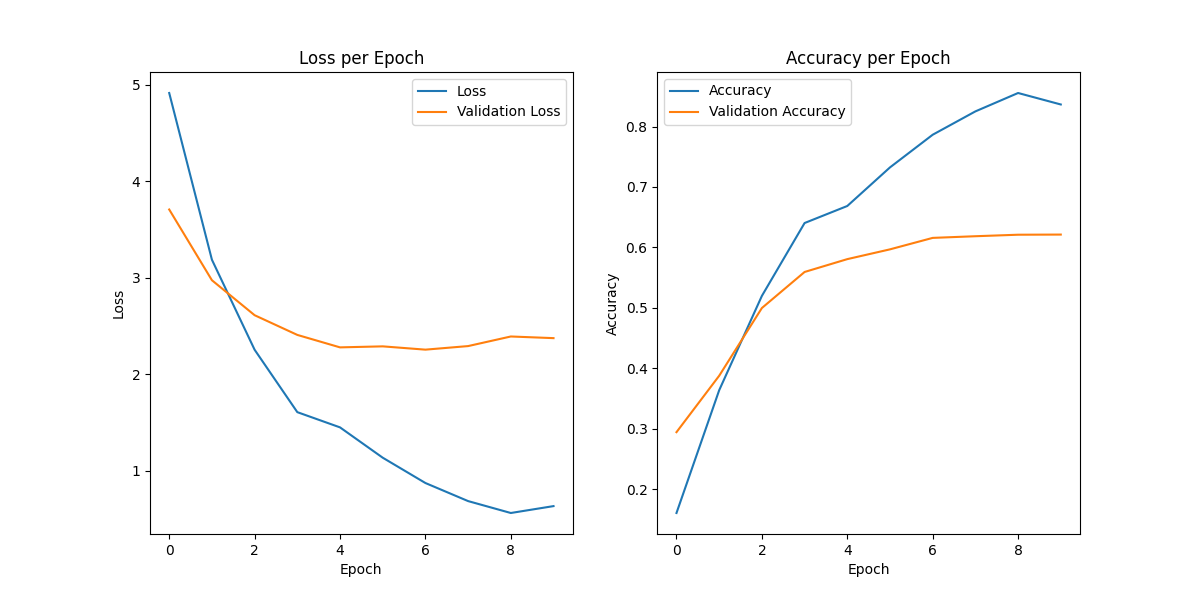
\includegraphics[width=\textwidth]{figures/training/learning_curve_fold_1.png}
        \caption{Fold 1}
        \label{fig:plot1}
    \end{subfigure}
    \hfill
    \begin{subfigure}[b]{0.4\textwidth}
        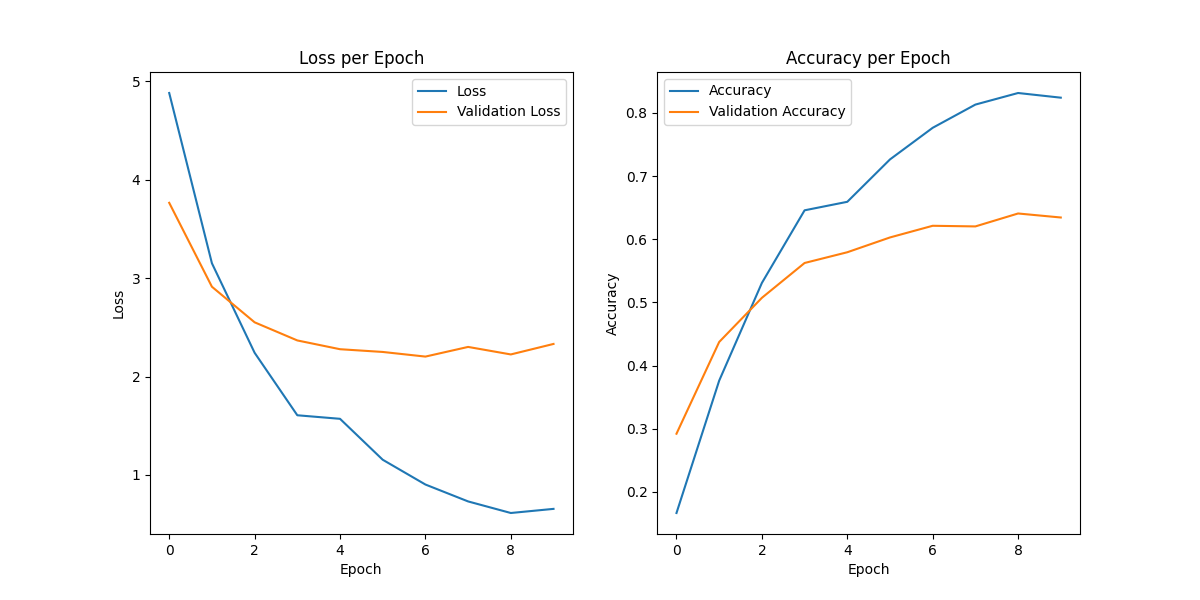
\includegraphics[width=\textwidth]{figures/training/learning_curve_fold_2.png}
        \caption{Fold 2}
        \label{fig:plot2}
    \end{subfigure}
    \hfill
    \begin{subfigure}[b]{0.4\textwidth}
        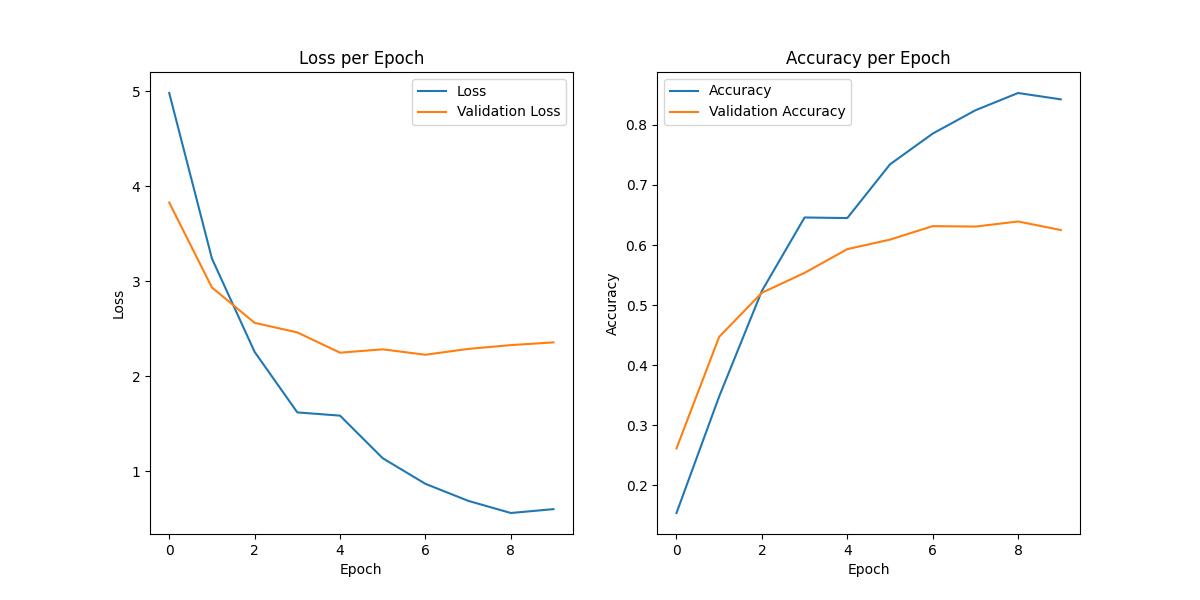
\includegraphics[width=\textwidth]{figures/training/learning_curve_fold_3.png}
        \caption{Fold 3}
        \label{fig:plot3}
    \end{subfigure}
    
    \vspace{1em}
    
    \begin{subfigure}[b]{0.4\textwidth}
        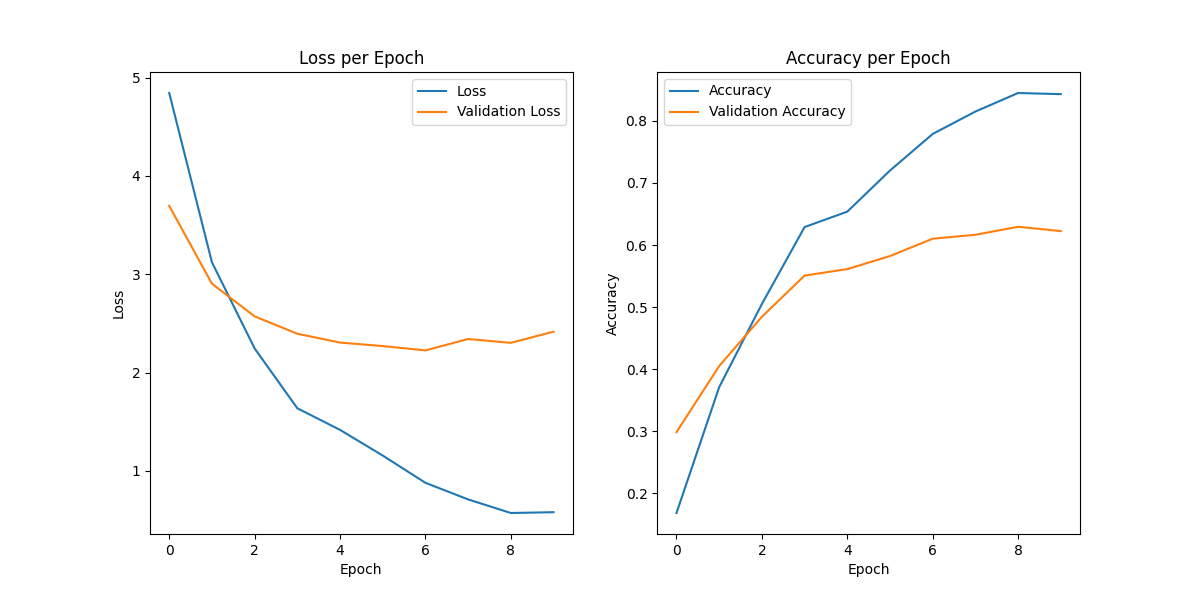
\includegraphics[width=\textwidth]{figures/training/learning_curve_fold_4.png}
        \caption{Fold 4}
        \label{fig:plot4}
    \end{subfigure}
    \hfill
    \begin{subfigure}[b]{0.4\textwidth}
        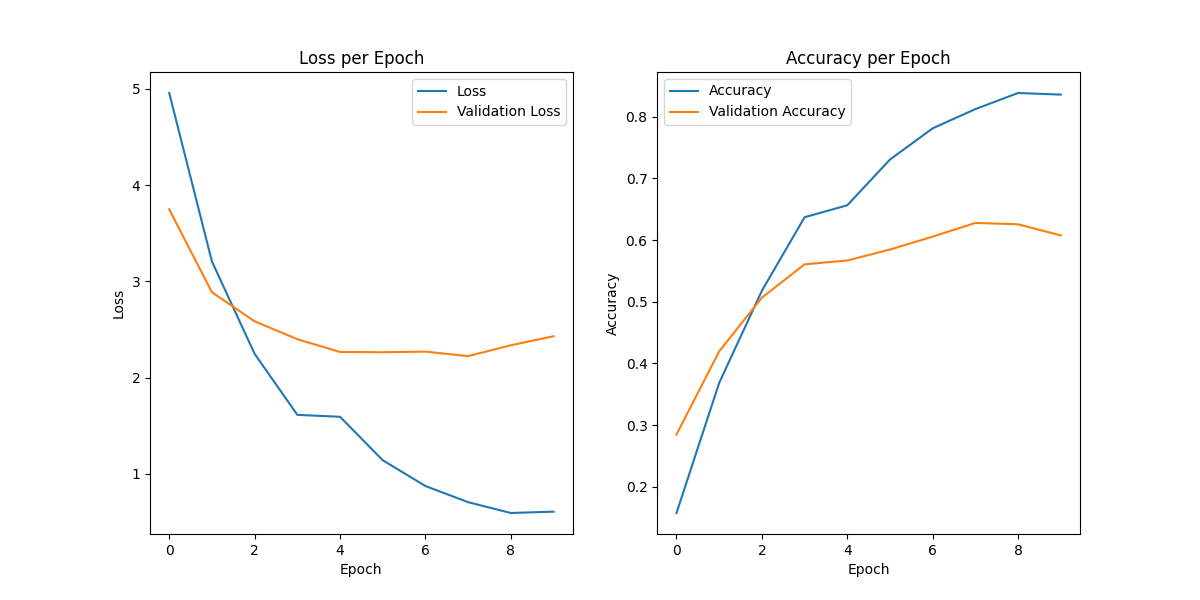
\includegraphics[width=\textwidth]{figures/training/learning_curve_fold_5.png}
        \caption{Fold 5}
        \label{fig:plot5}
    \end{subfigure}
    
    \caption{Learning curves for all 5 folds.}
    \label{fig:all_folds}
\end{figure}

From the plots, we can say that the model achieved overfit after 8 epochs
(the model is memorizing the training data rather than generalizing). 
Learning patterns in all 5 folds are similar, this indicates consistent 
performance across different data splits, suggesting the model is robust.
However, validation loss and validation accuracy curves significantly diverge from 
training curves. We suppose, this is due to our insufficient training data which is limited 
as we are limited by our datasets and only C programming language functions.

% average metrics table
\begin{figure}[h!]
    \centering
    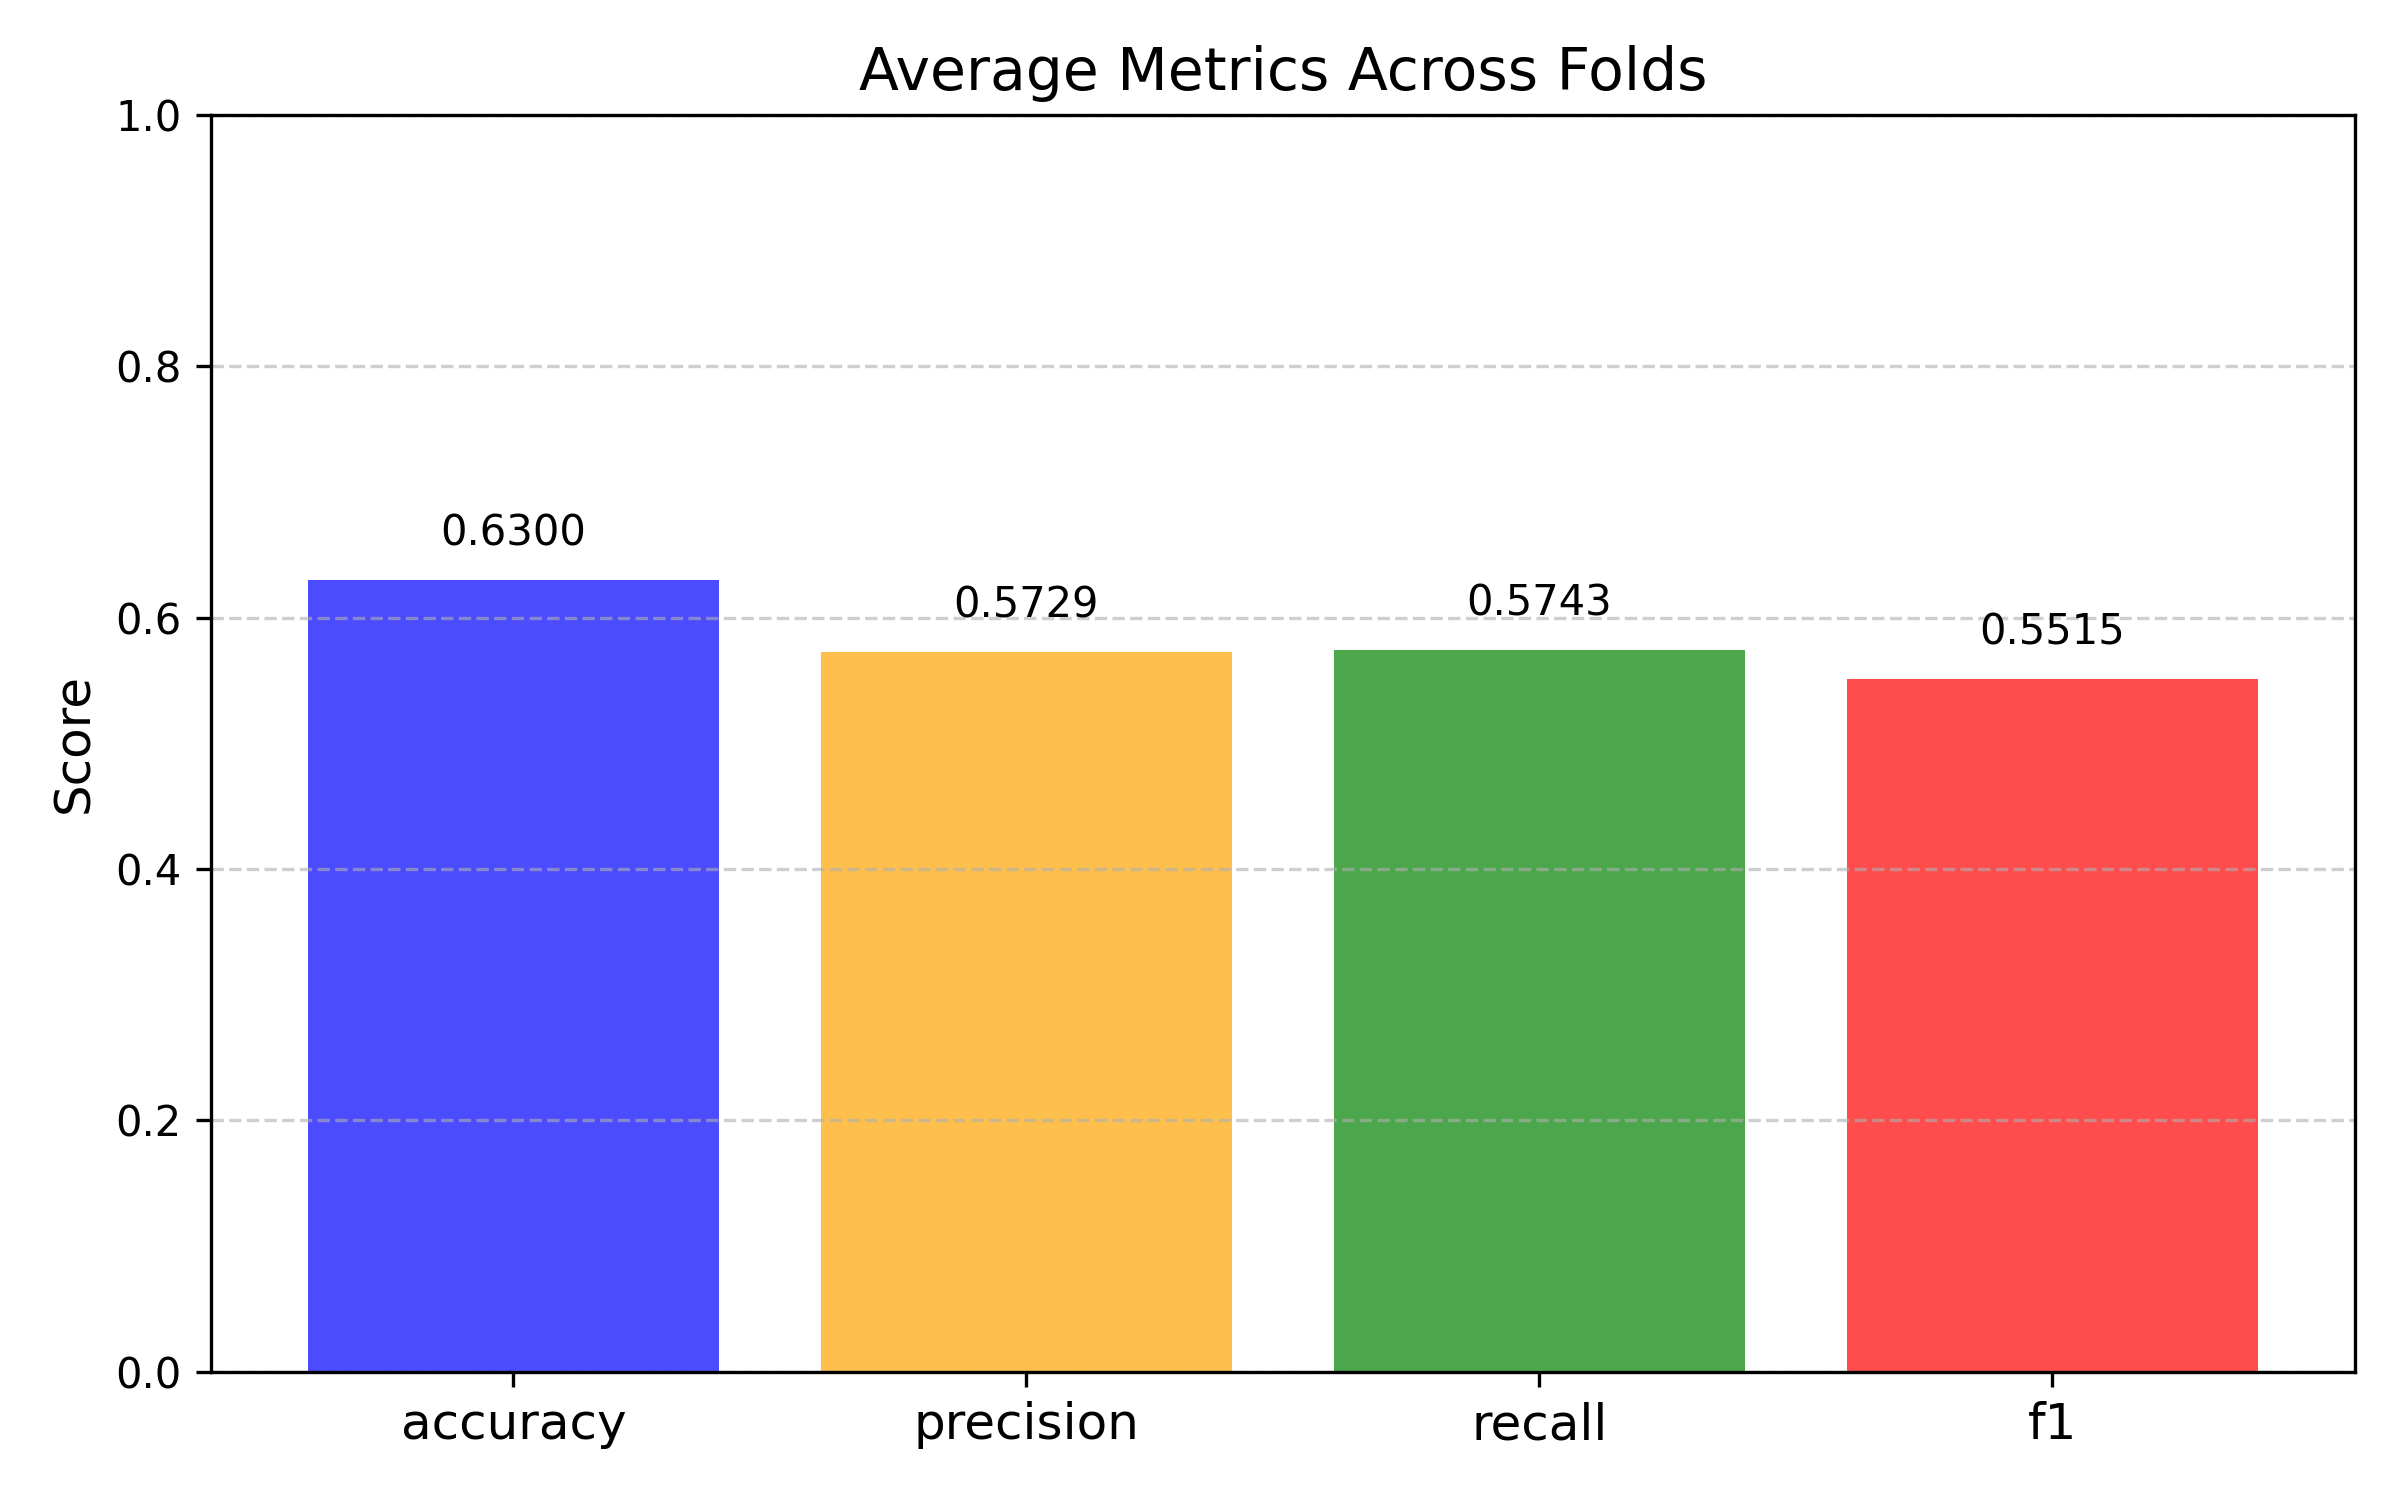
\includegraphics[width=8cm, height=4cm]{figures/testing/agg_average_metrics_plot.png} 
    \caption{Average testing metrics across folds.}
    \label{fig:average_testing_metrics}
\end{figure}


\subsubsection{Testing}

\begin{figure}[h!]
    \centering
    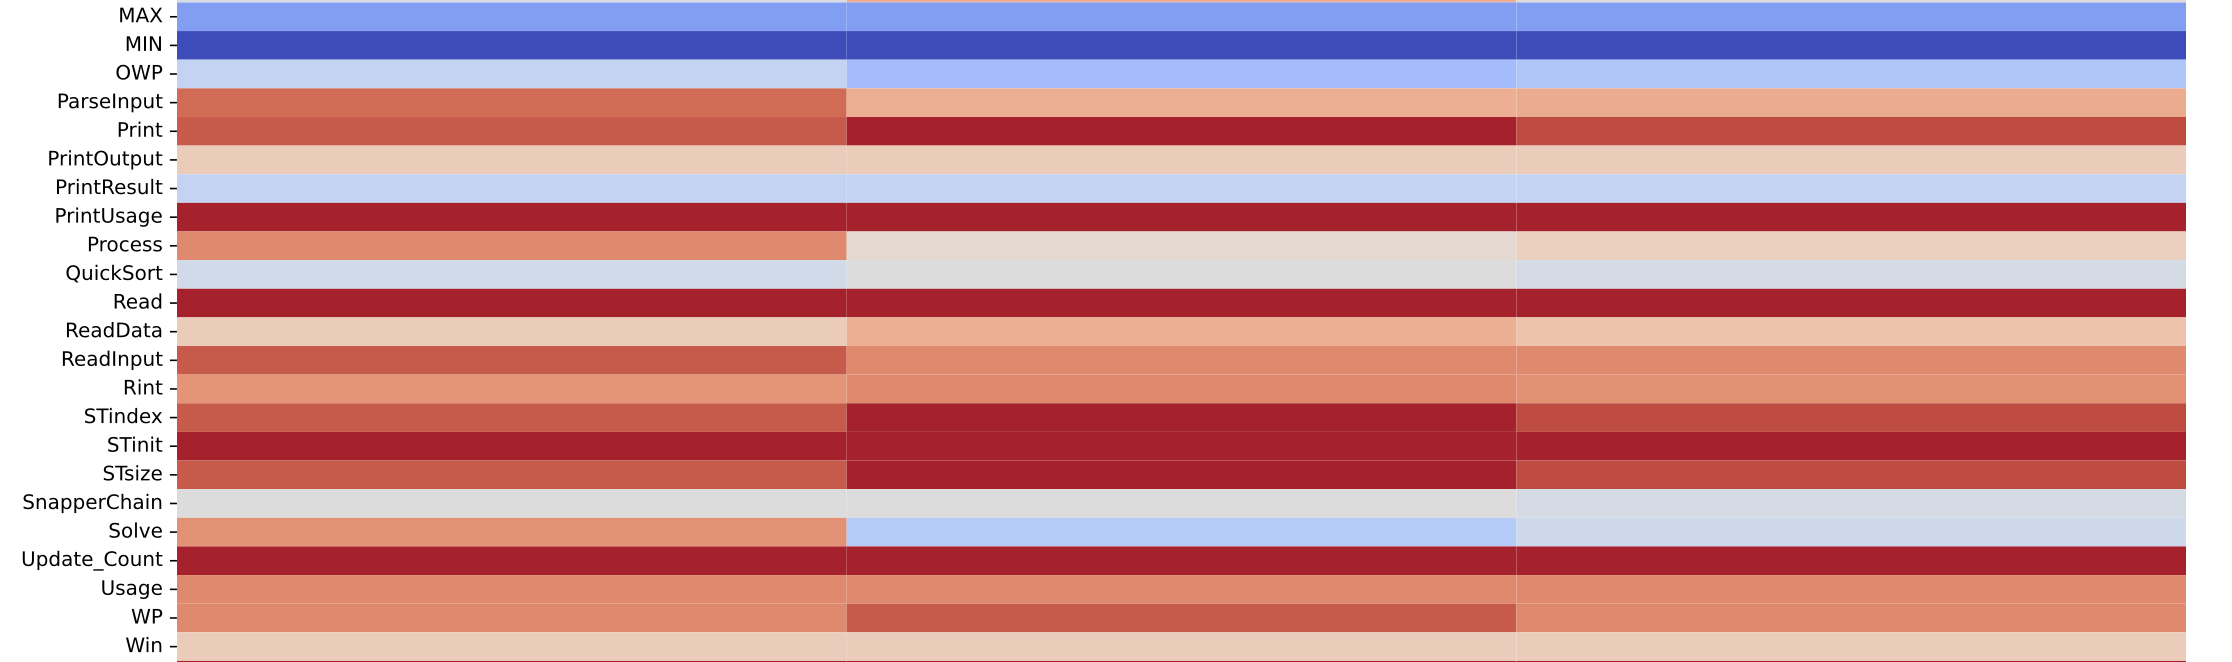
\includegraphics[width=16cm, height=6cm]{figures/heatmap_snippet.png} 
    \caption{Snippet from heatmap of names as classes.}
    \label{fig:func_lengths_distr_merged}
\end{figure}



\section{Extensive Data Preprocessing}




\bibliographystyle{plain}
\bibliography{references}
\end{document} 

